
\section{Unified Memory Analysis \cite{li2015evaluation}} \label{subsec:unifmemanaly}
An evaluation of Unified Memory is provided in \cite{li2015evaluation}.
It describes the Unified Memory programming model and presents an evaluation methodology to try to understand how the automatic system works.
It is known that the system handles data migration transparently, but the workflow is unknown.
The tests are carried on the K40 Accelerator and the Jetson TK1 (embedded).
The latter is interesting because it has physically unified memory.

To evaluate the performance, three different benchmarks are used.
One is the Matrix Multiplication benchmark.
It consists of tests with both cuBLAS and a block matrix multiplication that uses shared memory.
The second is the Diffussion 3D Benchmark.
The last one is the Parboil Benchmark Suite, created for studying the performance of computer architectures and compilers.
Only the benchmarks using a constant memory size are used.
The comparison is made by modifying them to use Unified Memory.
No optimization changes are made.
The tool used to analyze the different runs is the NVIDIA Profiler.
The Profiler provides a graphical interface breaking down the time consumption among sub-tasks, streams, etc.
It is also shown that the structure and content of PTX codes (pseudo-asssembly codes for CUDA) does not change.

\begin{figure}[ht!]
    \centering
    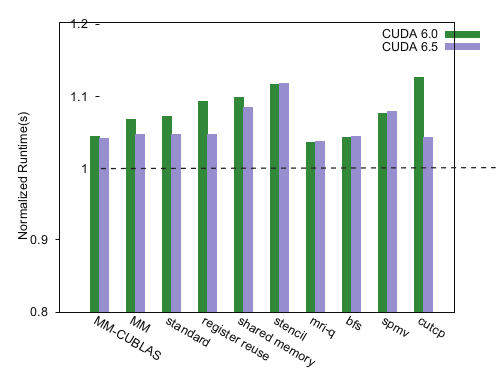
\includegraphics[width=\linewidth]{unified_memory_benchmark_results}
    \caption{Benchmark comparison results, where 1 is the runtime of the version without Unified Memory \cite{li2015evaluation}}
    \label{fig:umem}
\end{figure}

As seen in Figure \ref{fig:umem}, it is found that there are 10\% performance losses in average.
This is shown to be due to redundant memory transfers and page caching faults.
These losses are in some benchmarks considerably smaller under CUDA 6.5 than under CUDA 6.0.
The kernel running time in CUDA 6.5 does not improve.
It is the performance of launching and synchronizing what improves between both CUDA versions.
Interestingly, the Jetson TK1 uses the memory of CPU and GPU separately, even when it is physically one, resulting in uneeded copies.
It is also shown that pinned memory is used for Unified Memory.
This is revealed by the fact that copying times from host to device are much lower under Unified Memory.

Finally, five micro-benchmarks are created to look for the conditions causing the performance loss.
It is seen that memory is copied from host to device even if no kernel uses it.
Memory also gets copied back and forth even if it is only read by the GPU.
Only in the case that the CPU never reads or writes the data, are there no redundant memory transfers.

This same research group intends to analyze the performance under of Unified Memory in multi-GPU systems in the future.
These results should suffer very significant changes due to hardware support for page faulting and the higher speeds of NVLink.
